%%%%%%%%%%%%%%%%%%%%%%%%%%%%%%%%%%%%%%%%%%%%%%%%%%%%%%
% A Beamer template for University of Wollongong     %
% Based on THU beamer theme                          %
% Author: Qiuyu Lu                                   %
% Date: July 2024                                    %
% LPPL Licensed.                                     %
%%%%%%%%%%%%%%%%%%%%%%%%%%%%%%%%%%%%%%%%%%%%%%%%%%%%%%
% Customized for Sharif University of Technology     %
%%%%%%%%%%%%%%%%%%%%%%%%%%%%%%%%%%%%%%%%%%%%%%%%%%%%%%


\documentclass[serif, aspectratio=169]{beamer}
%\documentclass[serif]{beamer}  % for 4:3 ratio
\usepackage[T1]{fontenc} 
\usepackage{fourier} % see "http://faq.ktug.org/wiki/uploads/MathFonts.pdf" for other options
\usepackage{hyperref}
\usepackage{latexsym,amsmath,xcolor,multicol,booktabs,calligra}
\usepackage{graphicx,pstricks,listings,stackengine}
\usepackage{lipsum}
\usepackage[normalem]{ulem}
\usepackage{caption}
\usepackage{tikz}

\author{Ali Sharifi-Zarchi}
\title{Machine Learning (CE 40717)}
\subtitle{Fall 2024}
\institute{
    CE Department \\
    Sharif University of Technology
}
%\date{\small \today}
% \usepackage{UoWstyle}
\usepackage{SUTstyle}

% defs
\def\cmd#1{\texttt{\color{red}\footnotesize $\backslash$#1}}
\def\env#1{\texttt{\color{blue}\footnotesize #1}}
\definecolor{deepblue}{rgb}{0,0,0.5}
\definecolor{deepred}{RGB}{153,0,0}
\definecolor{deepgreen}{rgb}{0,0.5,0}
\definecolor{halfgray}{gray}{0.55}

\lstset{
    basicstyle=\ttfamily\small,
    keywordstyle=\bfseries\color{deepblue},
    emphstyle=\ttfamily\color{deepred},    % Custom highlighting style
    stringstyle=\color{deepgreen},
    numbers=left,
    numberstyle=\small\color{halfgray},
    rulesepcolor=\color{red!20!green!20!blue!20},
    frame=shadowbox,
}
\captionsetup{labelformat=empty}

\begin{document}

\begin{frame}
    \titlepage
    \vspace*{-0.6cm}
    \begin{figure}[htpb]
        \begin{center}
            
\includegraphics[keepaspectratio, scale=0.25]{pic/sharif-main-logo.png}
        \end{center}
    \end{figure}
    \vfill % This pushes the next content to the bottom
    \vspace{-0.35cm}
    % \centering\textit{\tiny Most slides are adapted from Dr. Mahdie Soleymani's ML course}
\end{frame}

\begin{frame}    
\tableofcontents[sectionstyle=show,
subsectionstyle=show/shaded/hide,
subsubsectionstyle=show/shaded/hide]
\end{frame}


\section{Introduction}

\begin{frame}{Classification problem}
    \begin{itemize}
        \item \textbf{Classification (binary)}
        \begin{itemize}
            \item Email: Spam / Not Spam?
            \item Online Transactions: Fraudulent / Genuine?
            \item Tumor: Malignant / Benign?
        \end{itemize}
    \end{itemize}
    
    
    \[
               \mathbf{y \in \{0, 1\} } \begin{cases}
                    & \text{0: ``Negative Class'' (e.g., benign tumor)} \\
                     & \text{1: ``Positive Class'' (e.g., malignant tumor)}
                \end{cases}
            \]
\end{frame}

\begin{frame}{Classification problem (cont.)}
    \begin{itemize}
        \item Can we solve the problem using linear regression?
    \end{itemize}
    
    \begin{minipage}{0.48\linewidth}
        \centering
        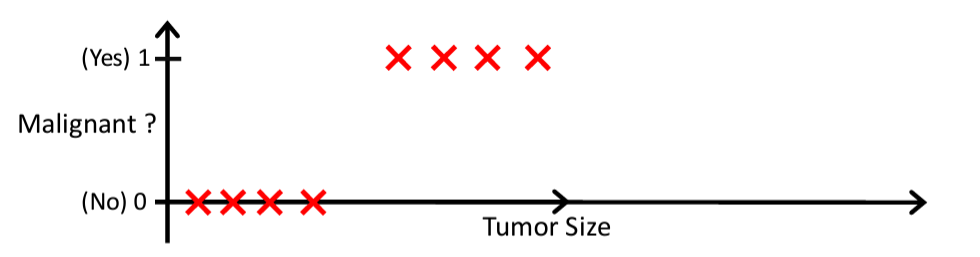
\includegraphics[width=\linewidth]{pic/lrClassification1.png}
    \end{minipage}
    \hfill
    \begin{minipage}{0.48\linewidth}
        \centering
        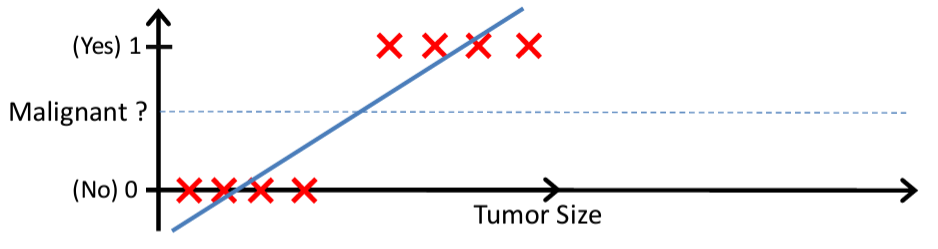
\includegraphics[width=\linewidth]{pic/lrClassification3.png}
    \end{minipage}
    
    \begin{itemize}
        \item We could fit a straight line and define a threshold at $0.5$:
            \begin{align*}
                & \textbf{If  } h_\theta (x) \geq 0.5, \text{predict  } y=1 \\
                & \textbf{If  } h_\theta (x) < 0.5, \text{predict  } y=0
            \end{align*}
    \end{itemize}
\end{frame}

%%%%%%%%%%%%%%%%
\begin{frame}{Classification problem (cont.)}
    \begin{itemize}
        \item What about now? (By adding a new data point)
    \end{itemize}
    
    \centering
    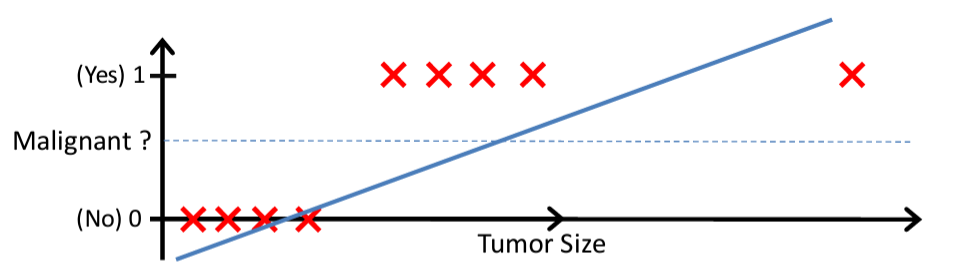
\includegraphics[width=0.68\linewidth]{pic/lrClassification2.png}
    
    \begin{itemize}
        \item Classification: $y=0$ or $y=1$
            \begin{itemize}
                \item $h_ \theta(x)$ can be $>1$ or $<0$
                \item Another drawback of using linear regression for this problem
            \end{itemize}
        \item What we need:
    \end{itemize}
    \begin{align*}
        \text{Logistic regression:  } 0 \leq h_\theta (x) \leq 1
    \end{align*}
    \begin{itemize}
        \item We also show this function with other notations: $f(x;w)= \sigma (w^Tx)$
    \end{itemize}
\end{frame}



\section{Logistic Regression}

\subsection{Fundamentals}


%%%% 5 %%%%%
\begin{frame}{Introduction}
    % \begin{itemize}
    %     \item Logistic regression is a \textbf{discriminative} approach.
    % \end{itemize}
    % \begin{figure}[h]
    %   \centering
    %   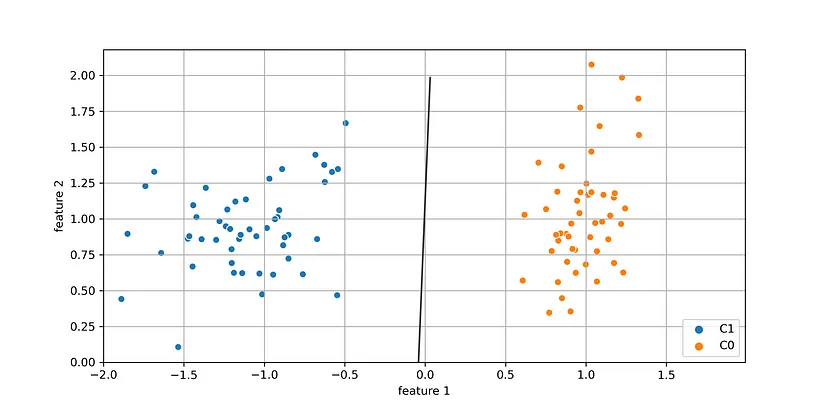
\includegraphics[width=0.6\textwidth]{pic/logisticR-Linear.png}
    %   % \label{fig:image}
    % \end{figure}
    \begin{itemize}
        \item Suppose we have a binary classification task (so $K=2$).
        \item By observing \textcolor{deepred}{age}, \textcolor{deepred}{gender}, \textcolor{deepred}{height}, \textcolor{deepred}{weight} and \textcolor{deepred}{BMI} we try to distinguish if a person is \textcolor{deepgreen}{overweight} or \textcolor{deepgreen}{not overweight}.
        
        
        %%%
        \begin{table}[h!]
        \centering
        \begin{tabular}{|c|c|c|c|c|c|}
        \hline
        \textcolor{deepred}{Age} & \textcolor{deepred}{Gender} & \textcolor{deepred}{Height (cm)} & \textcolor{deepred}{Weight (kg)} & \textcolor{deepred}{BMI} & \textcolor{deepgreen}{Overweight} \\ \hline
        25 & Male & 175 & 80 & 25.3 & 0 \\ \hline
        30 & Female & 160 & 60 & 22.5 & 0 \\ \hline
        \multicolumn{6}{|c|}{\dots} \\ \hline
        35 & Male & 180 & 90 & 27.3 & 1 \\ \hline
        \end{tabular}
        % \caption{Sample Table}
        % \label{tab:sample}
        \end{table}
        %%%%
        \item We denote the \textcolor{deepred}{features} of a sample with vector $x$ and the \textcolor{deepgreen}{label} with $y$.
        \item In logistic regression we try to find an $\sigma (w^Tx)$ which predicts \textbf{posterior} probabilities $P(y=1|x)$.
    \end{itemize}
    
\end{frame}
%%%% 5.1 %%%%%%%%%
\begin{frame}{Introduction (cont.)}
    \begin{itemize}
        \item $\sigma (w^Tx)$: probability that $y=1$ given $x$ (parameterized by \textbf{$\textbf{w}$})
      \begin{align*}
        P(y=1|x,\mathbf{w}) &= \sigma (\mathbf{w}^Tx) \\
        P(y=0|x,\mathbf{w}) &= 1 - \sigma (\mathbf{w}^Tx)
      \end{align*}

        \item We need to look for a function which gives us an output in the range [0, 1]. (like a probability).

        \item Let's denote this function with $\sigma (.)$ and call it the \textbf{activation function}.
        
    \end{itemize}
\end{frame}

%%%% 6 %%%%%
\begin{frame}{Introduction (cont.)}
    \begin{minipage}{0.55\textwidth}
    \begin{itemize}
        \item Sigmoid (logistic) function.
        \[
            \sigma (z) = \frac{1}{1 + e^{-z}}
        \]
        \item A good candidate for activation function.
        
        \item It gives us a number between 0 and 1 \textbf{smoothly}.
        \item It is also \textbf{differentiable}

    \end{itemize}
    \end{minipage}% 
    \begin{minipage}{0.4\textwidth}
        \centering
        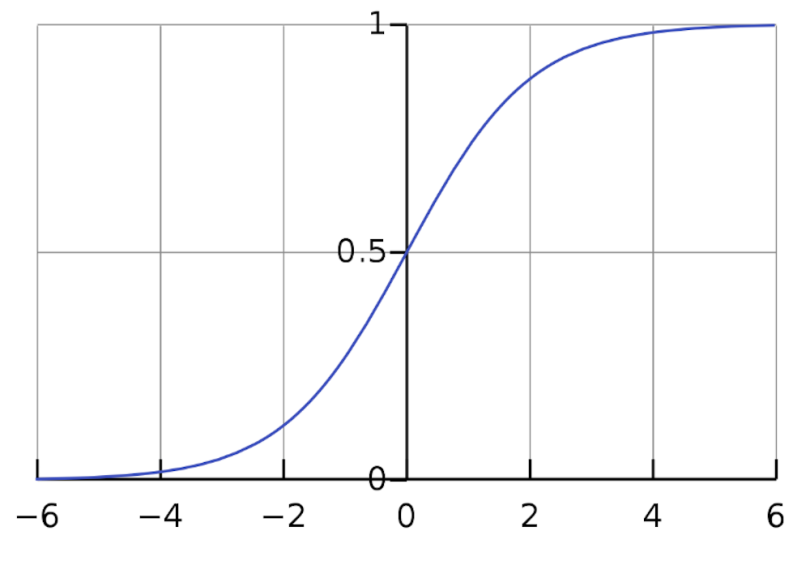
\includegraphics[width=0.8\textwidth]{pic/sigmoid.png}
    \end{minipage}
\end{frame}
%%%%%%%%%%%%%%%%%%%%%%%%%%%%%%%%%%%%%%%%
\begin{frame}{Sigmoid function \& its derivative}
    \centering
        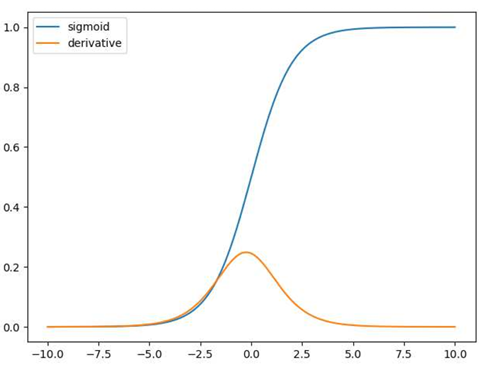
\includegraphics[width=0.65\textwidth]{pic/sigmoidDer.png}
\end{frame}

%%%%%%%%%%%%%%%%%%%%%%%%%%%%%%%%%%%%%%%%
%%%% 7 %%%%
% \begin{frame}{Basics Cont.}
%     \begin{itemize}
%       \item Sigmoid function plot
%       \begin{figure}[h]
    
%       % \caption{Sigmoid plot}
%     % \label{fig:image}
%     \end{figure}
%     \end{itemize}
% \end{frame}
%%%% 8 %%%%%
\begin{frame}{Introduction (cont.)}
    \begin{itemize}
      \item The sigmoid function takes a number as input but we have:
    \end{itemize}
        \begin{align*}
            x &= [x_0=1,x_1, \dots, x_d] \\
            w &= [w_0, w_1, \dots, w_d]
        \end{align*}
    \begin{itemize} 
      \item So we can use the \textbf{dot product} of $x$ and $w$.
      
      \item We have $0\leq \sigma (\mathbf{w}^Tx) \leq 1$. which is the estimated probability of $y=1$ on input $x$.

      \item An Example : A basketball game (Win, Lose)
        \begin{itemize}
            \item $\sigma (\mathbf{w}^T x) = 0.7$
            \item In other terms $70$ percent chance of winning the game.
        \end{itemize}
        
    \end{itemize}
\end{frame}
%%%%% 9 %%%%%%%
\subsection{Decision surface}
\begin{frame}{Decision surface}
    \begin{itemize}
      \item Decision surface or decision boundary is the region of a problem space in which the output label of a classifier is ambiguous. (could be linear or non-linear)
      \item In binary classification it is where the probability of a sample belonging to each $y=0$ and $y=1$ is equal.
    \end{itemize}
    
    
     \begin{center}
        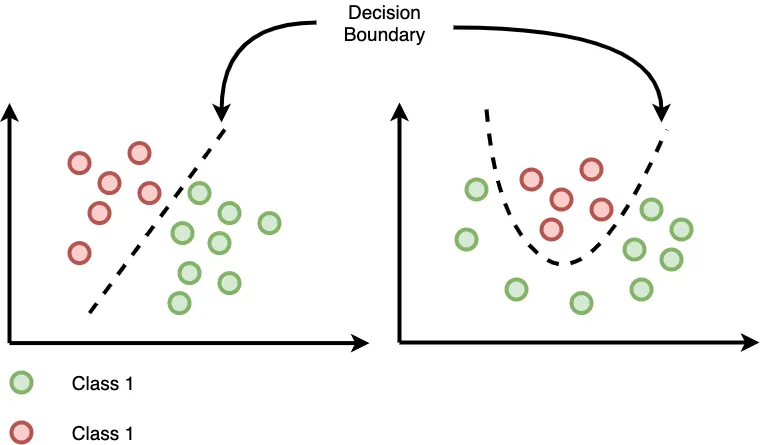
\includegraphics[width=0.4\textwidth]{pic/decision boundary.png}
        % \captionof{figure}{\footnotesize [Eric Xing, Machine Learning, CMU]}
    \end{center}
    
    \begin{itemize}
        
      \item Decision boundary hyperplane always has \textbf{one less dimension} than the feature space.
      
      
      %%% next slide
    %   \item an example of decision boundaries:
      
     
    \end{itemize}
\end{frame}
%%%%% 9.4 %%%%%%
\begin{frame}{Decision surface (cont.)}

    \begin{itemize}
        \item An example of linear decision boundaries:
    \end{itemize}
    \begin{center}
        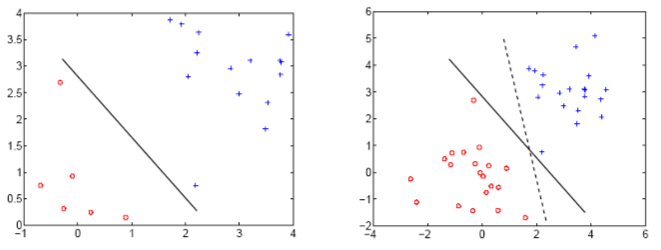
\includegraphics[width=0.85\textwidth]{pic/DBoundary.png}
        % \captionof{figure}{\footnotesize [Eric Xing, Machine Learning, CMU]}
    \end{center}
    \begin{tikzpicture}[remember picture,overlay]
        \node[anchor=south west, xshift=0.1cm, yshift=0.22cm] at (current page.south west) {
            \scriptsize Figure adapted from Eric Xing, Machine Learning, CMU
        };
    \end{tikzpicture}
\end{frame}
%%%% 9.5 %%%%%

\begin{frame}{Decision surface (cont.)}
    \begin{itemize}
      \item Back to our logistic regression problem.
      \item Decision surface $\sigma (\mathbf{w}^Tx) = $ \textbf{constant}.
        \[
            \sigma (\mathbf{w}^Tx) = \frac{1}{1 + e^{-(\mathbf{w}^Tx)}} = 0.5
        \]
      \item Decision surfaces are \textbf{linear functions} of $x$
        \begin{itemize}
            \item if $\sigma (\mathbf{w}^Tx) \geq 0.5$ then $\hat{y}=1$, else $\hat{y} = 0$
            \item Equivalently, if $\mathbf{w}^Tx + w_0 \geq 0.5$ then decide $\hat{y}=1$, else $\hat{y}=0$
        \end{itemize}% ayoub eshgh
        \vfill
        \begin{center}
            \( \hat{y} \) \textbf{is the predicted label}
        \end{center}
    \end{itemize}
\end{frame}

%%%% 10 %%%%
\begin{frame}{Decision boundary example}
    \begin{align*}
        \sigma (\mathbf{w}^Tx) = \sigma (w_0 + w_1 x_1 + w_2 x_2)
    \end{align*}
    
    \begin{minipage}{0.35\linewidth}
        \centering
        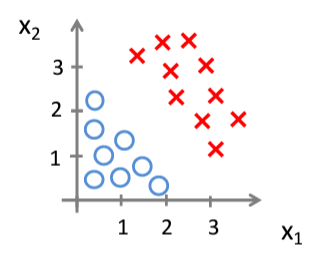
\includegraphics[width=\linewidth]{pic/lrDB1.png}
    \end{minipage}
    \hfill
    \begin{minipage}{0.35\linewidth}
        \centering
        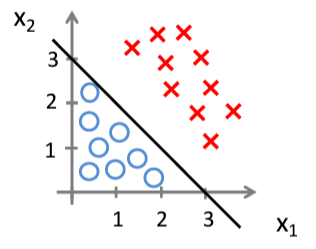
\includegraphics[width=\linewidth]{pic/lrDB2.png}
    \end{minipage}
    
    \begin{align*}
        \text{Predict } y=1 \text{ if } -3 + x_1 + x_2 \geq 0
    \end{align*}
    
\end{frame}
%%%%%%%%%%%%%
\begin{frame}{Non-linear decision boundary example}
    \begin{align*}
        \sigma (\mathbf{w}^Tx) &= \sigma (w_0 + w_1 x_1 + w_2 x_2 + w_3x_1^2 + w_4x_2^2) \\
        \text{We can learn } & \text{more complex decision boundaries when having higher order terms}
    \end{align*}
    
    \begin{minipage}{0.30\linewidth}
        \centering
        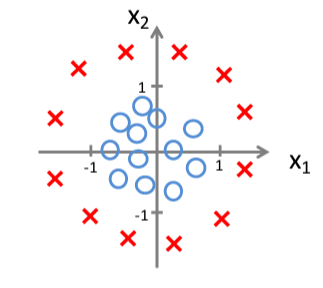
\includegraphics[width=\linewidth]{pic/lrDB3.png}
    \end{minipage}
    \hfill
    \begin{minipage}{0.30\linewidth}
        \centering
        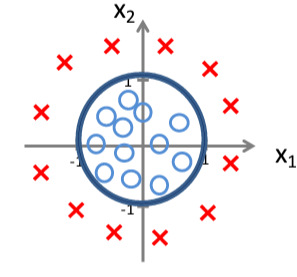
\includegraphics[width=\linewidth]{pic/lrDB4.png}
    \end{minipage}
    
    \begin{align*}
        \text{Predict } y=1 \text{ if } -1 + x_1^2 + x_2^2 \geq 0
    \end{align*}
    
\end{frame}
%%%%%%%%%%%%%
\subsection{ML estimation}

\begin{frame}{ML estimation}
    \begin{itemize}
        \item We had posterior of a sample as:
        \begin{align*}
            P(y^{(i)}|x^{(i)},\mathbf{w})
        \end{align*}
        \item Logistic regression should maximize production of all these sample posteriors.
        
        \item Maximum (conditional) log likelihood:
        \begin{align*}
             \mathbf{\hat{w}} = \underset{w}{\arg\max} \hspace{0.2cm} \log \prod_{i=1}^{n} P(y^{(i)}|x^{(i)},\mathbf{w})
        \end{align*}
        \item Note that in \textbf{binary} classification $y$ is either $1$ or $0$, So we can have posterior term simplified as follows:
        
        \begin{align*}
            P(y^{(i)}|x^{(i)},\mathbf{w})=\sigma (\mathbf{w}^Tx^{(i)})^{y^{(i)}} (1 - \sigma (\mathbf{w}^T x^{(i)}))^{(1 - y^{(i)})}
        \end{align*}
    \end{itemize}
\end{frame}
%%%%%% 10.5 %%%%%%%%%%
\begin{frame}{ML estimation}
    \begin{itemize}
        \item Logarithm of the posterior probability:
            \[
            \log P(y^{(i)}|x^{(i)}, \mathbf{w})=
            y^{(i)}\log (\sigma (\mathbf{w} ^T x^{(i)})) + 
            (1-y^{(i)})\log (1 - \sigma (\mathbf{w}^T x^{(i)}))
            \]
        \item Hence the log likelihood is as follows:
    \end{itemize}
    \[
    \log \prod _{i=1}^{n} P(y^{(i)}|x^{(i)}, \mathbf{w}) = \sum  _{i=1}^{n} \log P(y^{(i)}|x^{(i)}, \mathbf{w})
    \]
    \[
    = \sum_{i=1}^{n}[y^{(i)}\log ( \sigma (\mathbf{w} ^T x^{(i)})) + 
    (1-y^{(i)})\log (1 - \sigma (\mathbf{w} ^ T x^{(i)}))]
    \]
\end{frame}


%%%%% 11 %%%%%
\subsection{Cost function}
\begin{frame}{Cost function}
    \begin{itemize}
    \item We should find 
        \begin{align*}
            \mathbf{\hat{w}} = \underset{w}{\arg\min} \hspace{0.2cm} J(w)
        \end{align*}
        \item MLE finds parameters that best describe a classification problem so cost function should be negative of log likelihood term:
        \begin{align*}
            J(w) &= -\sum_{i=1}^{n} \log P(y^{(i)}|x^{(i)}, \mathbf{w})\\
            &= \sum_{i=1}^{n}-y^{(i)}\log (\sigma (\mathbf{w}^T x^{(i)})) - 
            (1-y^{(i)})\log (1 - \sigma (\mathbf{w}^T x^{(i)}))
        \end{align*}
        \item No closed form solution for $\nabla _w J(w) = 0$
        \item However $J(w)$ is \textbf{convex}.
    \end{itemize}
\end{frame}

%%%%% 11.5 %%%%%%%%%%
\begin{frame}{Cost function (cont.)}
    \begin{itemize}
    \item Convexity of $J(w)$ can easily be proved:
        \begin{itemize}
            \item We use the lemma that sum of several convex functions is still convex (you can prove it on your own).
            \item Each term in the summation is differentiable (twice).
            \item If you twice get derivative of (with respect to $\sigma$):
                \[
                    -y^{(i)}\log (\sigma (\mathbf{w}^T x^{(i)})) - 
            (1-y^{(i)})\log (1 - \sigma (\mathbf{w}^T x^{(i)}))
                \]
            \item You get:
                \[
                    \frac{y}{\sigma ^2} + \frac{1-y}{(1-\sigma )^2}
                \]
            \item Which for both $y=0$ and $y=1$ is positive.
            \item Each $\log P(y^{(i)}|x^{(i)}, \mathbf{w})$ is convex, hence the summation is convex as well.
        \end{itemize}
    \end{itemize}
\end{frame}
%%%%% 11.7 %%%%%%
\begin{frame}{Cost function (cont.)}
    \begin{itemize}
    \item Visualization of each binary cross entropy loss term:
    \end{itemize}
    \begin{center}
        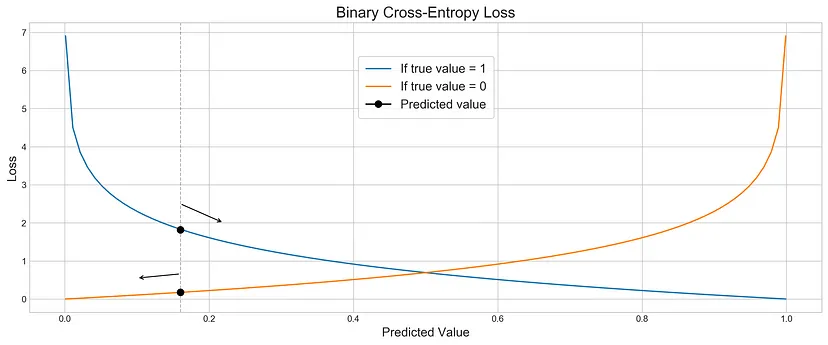
\includegraphics[width=0.7\textwidth]{pic/BCE2.png}
        % \captionof{figure}{\footnotesize [Eric Xing, Machine Learning, CMU]}
    \end{center}
    %% https://medium.com/@shrividya.gs/log-loss-penalty-for-overconfidence-ce8cb540eb45
    
    
    \begin{itemize}
        \item As you can see if the model predicted value is $\hat{y}=0.16$ and true label is $y=1$ then the error is high but if the true label is $y=0$ the error would be low.
    \end{itemize}
    \vfill
    \begin{tikzpicture}[remember picture,overlay]
    \node[anchor=south west, xshift=0.1cm, yshift=0.22cm] at (current page.south west) {
        \scriptsize Figure adopted from https://towardsdatascience.com/logistic-regression-from-scratch-69db4f587e17
    };
    \end{tikzpicture}
\end{frame}

%%%% 12 %%%%%%

\subsection{Gradient descent}
\begin{frame}{Gradient descent}
    \begin{itemize}
    \item Remember from previous slides:
        \[
        J(w) = \sum_{i=1}^{n}-y^{(i)}\log (\sigma (\mathbf{w}^T x^{(i)})) - 
            (1-y^{(i)})\log (1 - \sigma (\mathbf{w}^T x^{(i)}))
        \]
    \item Update rule for \textbf{gradient descent}: 
        \begin{align*}
            w^{t+1} = w^t - \eta \nabla _w J(w^t)
        \end{align*}
    \item With $J(w)$ definition for logistic regression we get:
        \begin{align*}
            \nabla _w J(w) = \sum_{i=1}^{n} (\sigma (\mathbf{w}^T x^{(i)}) - y^{(i)})x^{(i)} 
        \end{align*}
    % \item Also keep in mind $f(x^{(i)}; \mathbf{w})= \sigma (\mathbf{w}^Tx^{(i)})$
    % \item Compare with the gradient of \textbf{SSE} in \textbf{linear regression} :
    %     \begin{align*}
    %         \nabla _w J(w) = \sum_{i=1}^{n} (w^Tx^{(i)} - y^{(i)})x^{(i)}
    %     \end{align*}
        
    \end{itemize}
\end{frame}
%%%%%% 12.5 %%%%%%%
\begin{frame}{Gradient descent}
    \begin{itemize}
    
    \item Compare the gradient of \textcolor{deepgreen}{logistic regression} with the gradient of \textcolor{blue}{SSE} in \textcolor{blue}{linear regression} :
    \end{itemize}
        \begin{align*}
        \color{deepgreen}
             \nabla _w J(w) = \sum_{i=1}^{n} (\sigma (\mathbf{w}^Tx^{(i)}) - y^{(i)})x^{(i)} 
        \end{align*}
        \begin{align*}
            \color{blue}
            \nabla _w J(w) = \sum_{i=1}^{n} (\mathbf{w}^Tx^{(i)} - y^{(i)})x^{(i)}
        \end{align*}
        
\end{frame}

%%%%% 13 %%%%%%%%

\begin{frame}{Loss function}
    \begin{itemize}
        %% delete paranthesis
        \item Loss function is a single overall measure of loss incurred for taking our decisions (over entire dataset).
        \item We have:
        \[ Loss(y, \sigma (\mathbf{w}^T x)) = -y \times \log (\sigma ( \mathbf{w}^T x)) - (1-y) \times \log 
        (1 - \sigma (\mathbf{w}^T x))
        \]
        
        \item Since in binary classification either $y=1$ or $y=0$ we have:
            \[
                Loss(y, \sigma (\mathbf{w}^T x)) = \begin{cases}
                    - \log (\sigma (\mathbf{w}^T x)) & \textbf{if } y = 1 \\
                    - \log (1 - \sigma (\mathbf{w}^T x)) & \textbf{if } y = 0
                \end{cases}
            \]
        \item How is it related to zero-one loss? ($\hat{y}$ is the predicted label and $y$ is the ture label)
           \[
               Loss(y, \hat{y}) =  \begin{cases}
                    1 & \textbf{if } y \neq \hat{y} \\
                    0 & \textbf{if } y = \hat{y}
                \end{cases}
            \]
    \end{itemize}
\end{frame}

%%%%% 14 %%%%%%
% \begin{frame}{Cost Function Summary}
%     \begin{itemize}
%         \item Logistic regression (LR) has a more proper cost function for classification than SSE and Perceptron.

%         \item Why is the cost function of LR also more suitable than 
%             \begin{align*}
%                 J(w) = \frac{1}{n}\sum_{i=1}^{n}(y^{(i)} - f(x^{(i)}; \mathbf{w}))^2
%             \end{align*}
%         Where $f(x; \mathbf{w}) = \sigma(\mathbf{w}^Tx)$?
%             \begin{itemize}
%                 \item The conditional distribution $p(y|x, \mathbf{w})$ in the classification problem is not Guassian (it is \textbf{Bernoulli}).
%                 \item The cost function of LR is also convex.
%             \end{itemize}
%     \end{itemize}
% \end{frame}

%%%%%% 15 %%%%%%%

\subsection{Multi-class logistic regression}
\begin{frame}{Multi-class logistic regression}
    \begin{itemize}
        \item Now consider a problem where we have $K$ classes and every sample only belongs to one class (for simplicity).
        % \item For each class $k$, $f_k(x; \mathbf{W})$ predicts the probability of $y=k$.
        %     \begin{itemize}
        %         \item i.e., $P(y=k|x, \mathbf{W})$
        %     \end{itemize}
        % \item For each data point $x_0$, $\sum _{k=1}^{K} p(y=k|x_0, \mathbf{W})$ must be $1$
        %     \begin{itemize}
        %         \item $W$ denotes a matrix of $w_i$'s in which each $w_i$ is a weight vector dedicated for class label $i$.
        %     \end{itemize}
        % \item On a new input $x$, to make a prediction, we pick the class that maximizes $f_k(x; \mathbf{W})$:
        %     \begin{align*}
        %         \alpha (x) &= \underset{k=1, \dots , K}{\arg\max} \hspace{0.2cm} f_k(x) 
        %     \end{align*}
        %     \begin{center}
        %         \textbf{if $\color{red} f_k(x) > f_j(x)$ $\color{red} \forall j \neq k$ then decide $\color{red} C_k$}
        %     \end{center}
    \end{itemize}
    \centering
    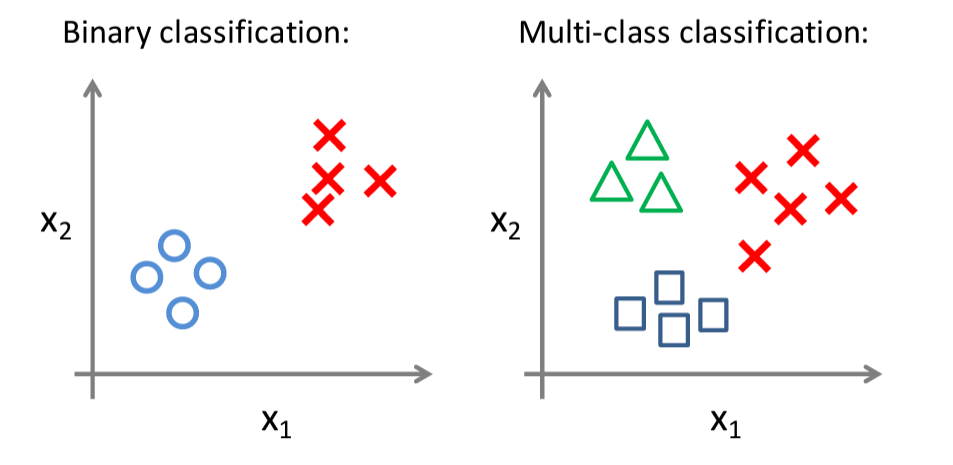
\includegraphics[width=0.8 \linewidth]{pic/multiVsBinaryC.png}
\end{frame}
%%%%%%%%%%%%%%%%%%%%%%%%
\begin{frame}{Multi-class logistic regression (cont.)}
    \begin{itemize}
         \item For each class $k$, $\sigma _k(x; \mathbf{W})$ predicts the probability of $y=k$.
            \begin{itemize}
                \item i.e., $P(y=k|x, \mathbf{W})$
            \end{itemize}
        \item For each data point $x_0$, $\sum _{k=1}^{K} P(y=k|x_0, \mathbf{W})$ must be $1$
            \begin{itemize}
                \item $W$ denotes a matrix of $w_i$'s in which each $w_i$ is a weight vector dedicated for class label $i$.
            \end{itemize}
        \item On a new input $x$, to make a prediction, we pick the class that maximizes $\sigma _k(x; \mathbf{W})$:
            \begin{align*}
                \alpha (x) &= \underset{k=1, \dots , K}{\arg\max} \hspace{0.2cm} \sigma _k(x; \mathbf{W}) 
            \end{align*}
            \begin{center}
                \textbf{if $\color{red} \sigma _k(x; \mathbf{W}) > \sigma _j(x; \mathbf{W})$ $\color{red} \forall j \neq k$ then decide $\color{red} C_k$}
            \end{center}
    \end{itemize}
\end{frame}


%%%%% 16 %%%%%%%
\begin{frame}{Multi-class logistic regression (cont.)}
    \begin{itemize}
        \item $K > 2$ and $y \in \{1,2,\dots,K\}$
        \begin{align*}
            \sigma _k(x, \mathbf{W}) = P(y=k|x) = \frac{\exp{(w^T_kx)}}{\sum_{j=1}^{K}\exp{(w_j^Tx)}}
        \end{align*}
        \item Normalized exponential (Aka \textbf{Softmax})
          
            \item if $w_k^Tx \gg w_j^Tx$ for all $j \neq k$ then $P(C_k|x) \approx 1$ and $P(C_j|x) \approx 0$
            \item Note : remember from Bayes theorem:
                \[
                P(C_k|x) = \frac{P(x|C_k)P(C_k)}
            {\sum_{j=1}^{K}P(x|C_j)P(C_j)}
                \]
          
    \end{itemize}
\end{frame}
%%%%% 16.5 %%%%%
\begin{frame}{Multi-class logistic regression (cont.)}
    \begin{itemize}
        \item Softmax function \textbf{smoothly} highlights the maximum probability and is differentiable.
        \item Compare it with $\max (.)$ function which is strict and non-differentiable
        \item Softmax can also handle negative values because we are using exponential function
        \item And it gives us probability for each class since:
            \begin{align*}
                \displaystyle \sum _{k=1}^{K} \frac{\exp (w_k^Tx)}{\sum _{j=1}^{K} \exp (w_j^Tx) } = 1
            \end{align*}
    \end{itemize}
\end{frame}

%%%% 16.6 %%%%%
\begin{frame}{Multi-class logistic regression (cont.)}
    \begin{itemize}
        \item An example of applying softmax (note that $z_i=w^Tx_i$):
    \end{itemize}
    \begin{center}
        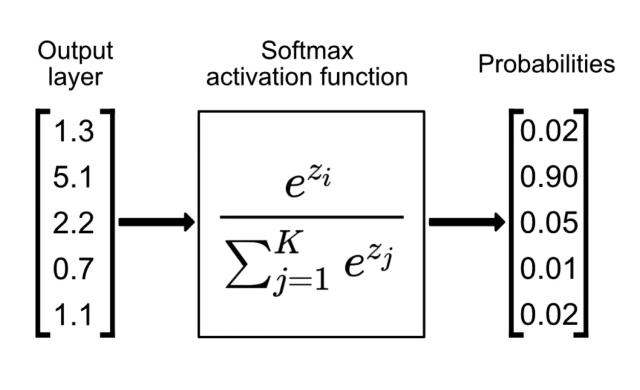
\includegraphics[width=0.7\textwidth]{pic/softmax0.png}
       
    \end{center}
\end{frame}

%%%% 17 %%%%%
\begin{frame}{Multi-class logistic regression (cont.)}
    \begin{itemize}
        \item Again we set $J(W)$ as negative of log likelihood.
        \item We need $\hat{W} = \underset{W}{\arg\min} \hspace{0.2cm} J(W)$
        \begin{align*}
            J(W) &= -\log \prod_{i=1}^{n} \textcolor{red}{P(y^{(i)}|x^{(i)}, \mathbf{W})} \\
            &= -\log \prod_{i=1}^{n}\textcolor{red}{\prod_{k=1}^{K}\sigma _k(x^{(i)}; \mathbf{W})^{y_k^{(i)}} }\\
            &= -\sum_{i=1}^{n}\sum_{k=1}^{K}y_k^{(i)} \log (\sigma _k(x^{(i)}; \mathbf{W}))
        \end{align*}
        \item If \textbf{$\textbf{i}$-th} sample belongs to class $k$ then $y^{(i)}_k$ is 1 else 0.
        \item Again no closed-from solution for $\hat{W}$
    \end{itemize}
    
\end{frame}
%%%%%%% 17.5 %%%%%%%
\begin{frame}{Multi-class logistic regression (cont.)}
    \begin{itemize}
        \item From previous slides we have:
            \begin{align*}
                J(W) = -\sum_{i=1}^{n}\sum_{k=1}^{K}y_k^{(i)} \log (\sigma _k(x^{(i)}; \mathbf{W}))
            \end{align*}
        \item In which:
             \[
        W = [w_1,w_2, \dots, w_K], \quad Y = 
        \text{\small $
        \begin{pmatrix}
            y^{(1)} \\
            y^{(2)} \\
            \vdots \\
            y^{(n)}
        \end{pmatrix}
        $}
        =
        \begin{pmatrix}
            y_1^{(1)} & \dots & y_K^{(1)} \\
            y_1^{(2)} & \dots & y_K^{(2)} \\
            \vdots    & \ddots & \vdots \\
            y_1^{(n)} & \dots & y_K^{(n)}
        \end{pmatrix}
    \]
    
        \item $y$ is a vector of length $K$ (1-of-$K$ encoding)
            \begin{itemize}
                % \item Each vector $y^{(i)}$ only consists of zeros and ones.
                \item For example $y=[0,0,1,0]^T$ when the target class is $C_3$.
            \end{itemize}
    \end{itemize}
\end{frame}
%%%%%% 18 %%%%%%%%
\begin{frame}{Multi-class logistic regression (cont.)}
    \begin{itemize}
        \item Update rule for gradient descent:
        
    \end{itemize}
    \begin{align*}
            w_j^{t+1} &= w_j^t - \eta \nabla _W J(W^t) \\
            \nabla _{w_{j}} J(W) &= \sum_{i=1}^{n} (\sigma _j(x^{(i)}; \mathbf{W}) - y_j^{(i)})x^{(i)}
        \end{align*}
        
    \begin{itemize}
        \item $w_j^t$ denotes the weight vector for class $j$ (since in multi-class LR, each class has its own weight vector) in the $t$-th iteration
    \end{itemize}
\end{frame}


\section{Summary}

\begin{frame}{Logistic regression (LR) summary}
    \begin{itemize}
        \item LR is a \textbf{linear} classifier
        \item LR optimization problem is obtained by \textbf{maximum likelihood}
            % \begin{itemize}
            %     \item when assuming \textbf{Bernoulli} distribution for conditional probabilities whose mean is $\frac{1}{1 + e^{-(w^Tx)}}$
            % \end{itemize}
        \item No closed-form solution for its optimization problem
            \begin{itemize}
                \item But convex cost function and global optimum can be found by gradient ascent
            \end{itemize}
    \end{itemize}
\end{frame}


% \section{Methods}

% \subsection{Diffusion Model}

% \begin{frame}{Title}
%     \begin{itemize}
%         \item \lipsum[3][1-4]
%     \end{itemize}
%     \begin{table}[h]
%         \centering
%         \begin{tabular}{c|c}
%             Microsoft\textsuperscript{\textregistered}  Windows & Apple\textsuperscript{\textregistered}  Mac OS \\
%             \hline
%             Windows-Kernel & Unix-like \\
%             Arm, Intel & Intel, Apple Silicon \\
%             Sudden update & Stable update \\
%             Less security & More security \\
%             ... & ... \\
%         \end{tabular}
%     \end{table}
% \end{frame}

% \begin{frame}{Algorithms}
%     \begin{exampleblock}{Non-Numbering Formula}
%         \begin{equation*}
%             J(\theta) = \mathbb{E}_{\pi_\theta}[G_t] = \sum_{s\in\mathcal{S}} d^\pi (s)V^\pi(s)=\sum_{s\in\mathcal{S}} d^\pi(s)\sum_{a\in\mathcal{A}}\pi_\theta(a|s)Q^\pi(s,a)
%         \end{equation*}
%     \end{exampleblock}
%     \begin{exampleblock}{Multi-Row Formula\footnote{If text appears in the formula,use $\backslash$mathrm\{\} or $\backslash$text\{\} instead}}
%         \begin{align}
%             Q_\mathrm{target}&=r+\gamma Q^\pi(s^\prime, \pi_\theta(s^\prime)+\epsilon)\\
%             \epsilon&\sim\mathrm{clip}(\mathcal{N}(0, \sigma), -c, c)\nonumber
%         \end{align}
%     \end{exampleblock}
% \end{frame}

% \begin{frame}
%     \begin{exampleblock}{Numbered Multi-line Formula}
%         % Taken from Mathmode.tex
%         \begin{multline}
%             A=\lim_{n\rightarrow\infty}\Delta x\left(a^{2}+\left(a^{2}+2a\Delta x+\left(\Delta x\right)^{2}\right)\right.\label{eq:reset}\\
%             +\left(a^{2}+2\cdot2a\Delta x+2^{2}\left(\Delta x\right)^{2}\right)\\
%             +\left(a^{2}+2\cdot3a\Delta x+3^{2}\left(\Delta x\right)^{2}\right)\\
%             +\ldots\\
%             \left.+\left(a^{2}+2\cdot(n-1)a\Delta x+(n-1)^{2}\left(\Delta x\right)^{2}\right)\right)\\
%             =\frac{1}{3}\left(b^{3}-a^{3}\right)
%         \end{multline}
%     \end{exampleblock}
% \end{frame}

% \begin{frame}{Graphics and Columns}
%     \begin{minipage}[c]{0.3\linewidth}
%         \psset{unit=0.8cm}
%         \begin{pspicture}(-1.75,-3)(3.25,4)
%             \psline[linewidth=0.25pt](0,0)(0,4)
%             \rput[tl]{0}(0.2,2){$\vec e_z$}
%             \rput[tr]{0}(-0.9,1.4){$\vec e$}
%             \rput[tl]{0}(2.8,-1.1){$\vec C_{ptm{ext}}$}
%             \rput[br]{0}(-0.3,2.1){$\theta$}
%             \rput{25}(0,0){%
%             \psframe[fillstyle=solid,fillcolor=lightgray,linewidth=.8pt](-0.1,-3.2)(0.1,0)}
%             \rput{25}(0,0){%
%             \psellipse[fillstyle=solid,fillcolor=yellow,linewidth=3pt](0,0)(1.5,0.5)}
%             \rput{25}(0,0){%
%             \psframe[fillstyle=solid,fillcolor=lightgray,linewidth=.8pt](-0.1,0)(0.1,3.2)}
%             \rput{25}(0,0){\psline[linecolor=red,linewidth=1.5pt]{->}(0,0)(0.,2)}
% %           \psRotation{0}(0,3.5){$\dot\phi$}
% %           \psRotation{25}(-1.2,2.6){$\dot\psi$}
%             \psline[linecolor=red,linewidth=1.25pt]{->}(0,0)(0,2)
%             \psline[linecolor=red,linewidth=1.25pt]{->}(0,0)(3,-1)
%             \psline[linecolor=red,linewidth=1.25pt]{->}(0,0)(2.85,-0.95)
%             \psarc{->}{2.1}{90}{112.5}
%             \rput[bl](.1,.01){C}
%         \end{pspicture}
%     \end{minipage}\hspace{2cm}
%     \begin{minipage}{0.5\linewidth}
%         \medskip
%         % \hspace{2cm}
%         \begin{figure}[h]
%             \centering
%             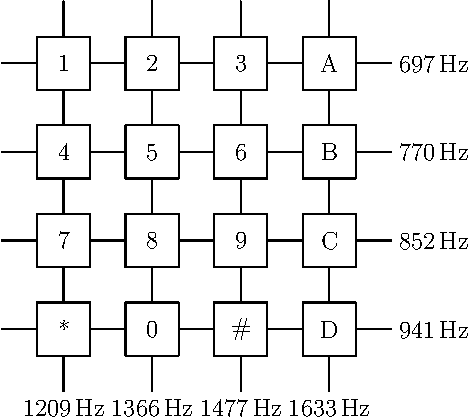
\includegraphics[height=.4\textheight]{pic/sample.pdf}
%         \end{figure}
%     \end{minipage}
% \end{frame}

% \begin{frame}[fragile]{\LaTeX{} Common Commands}
%     \begin{exampleblock}{Commands}
%         \centering
%         \footnotesize
%         \begin{tabular}{llll}
%             \cmd{chapter} & \cmd{section} & \cmd{subsection} & \cmd{paragraph} \\
%             chapter & section & sub-section & paragraph \\\hline
%             \cmd{centering} & \cmd{emph} & \cmd{verb} & \cmd{url} \\
%             center & emphasize & original & hyperlink \\\hline
%             \cmd{footnote} & \cmd{item} & \cmd{caption} & \cmd{includegraphics} \\
%             footnote & list item & caption & insert image \\\hline
%             \cmd{label} & \cmd{cite} & \cmd{ref} \\
%             label & citation & refer\\\hline
%         \end{tabular}
%     \end{exampleblock}
%     \begin{exampleblock}{Environment}
%         \centering
%         \footnotesize
%         \begin{tabular}{lll}
%             \env{table} & \env{figure} & \env{equation}\\
%             table & figure & formula \\\hline
%             \env{itemize} & \env{enumerate} & \env{description}\\
%             non-numbering item & numbering item & description \\\hline
%         \end{tabular}
%     \end{exampleblock}
% \end{frame}

% \begin{frame}[fragile]{\LaTeX{} Examples of environmental commands}
%     \begin{minipage}{0.5\linewidth}
% \begin{lstlisting}[language=TeX]
% \begin{itemize}
%   \item A \item B
%   \item C
%   \begin{itemize}
%     \item C-1
%   \end{itemize}
% \end{itemize}
% \end{lstlisting}
%     \end{minipage}\hspace{1cm}
%     \begin{minipage}{0.3\linewidth}
%         \begin{itemize}
%             \item A
%             \item B
%             \item C
%             \begin{itemize}
%                 \item C-1
%             \end{itemize}
%         \end{itemize}
%     \end{minipage}
%     \medskip
%     \pause
%     \begin{minipage}{0.5\linewidth}
% \begin{lstlisting}[language=TeX]
% \begin{enumerate}
%   \item A \item B
%   \item C
%   \begin{itemize}
%     \item[n+e]
%   \end{itemize}
% \end{enumerate}
% \end{lstlisting}
%     \end{minipage}\hspace{1cm}
%     \begin{minipage}{0.3\linewidth}
%         \begin{enumerate}
%             \item A
%             \item B
%             \item C
%             \begin{itemize}
%                 \item[n+e]
%             \end{itemize}
%         \end{enumerate}
%     \end{minipage}
% \end{frame}

% \begin{frame}[fragile]{\LaTeX{} Formulas}
%     \begin{columns}
%         \begin{column}{.55\textwidth}
% \begin{lstlisting}[language=TeX]
% $V = \frac{4}{3}\pi r^3$

% \[
%   V = \frac{4}{3}\pi r^3
% \]

% \begin{equation}
%   \label{eq:vsphere}
%   V = \frac{4}{3}\pi r^3
% \end{equation}
% \end{lstlisting}
%         \end{column}
%         \begin{column}{.4\textwidth}
%             $V = \frac{4}{3}\pi r^3$
%             \[
%                 V = \frac{4}{3}\pi r^3
%             \]
%             \begin{equation}
%                 \label{eq:vsphere}
%                 V = \frac{4}{3}\pi r^3
%             \end{equation}
%         \end{column}
%     \end{columns}
%     \begin{itemize}
%         \item more information \href{https://ja.overleaf.com/learn/latex/Mathematical_expressions}{\color{purple}{here}}
%     \end{itemize}
%%%%%%%%%%%%%%%%%%%%%%%%%%%%%%%%%%%%%%%%%%%%%%%%
\section{Extra reading}
\subsection{Probabilistic view in classification}
%%%% 0 %%%%%

% \begin{frame}{Probabilistic view in classification problem}
%     \begin{itemize}
%         \item First consider a simple classification problem:
%             \begin{itemize}
%                 \item We want to find individuals with diabetes and detect them.
%                 \item We have two \textbf{observations}: blood cell count and Plasma glucose value.
%                 \item Observations are our \textbf{features} and having Diabetes or not is our \textbf{class label} in this classification problem.
%             \end{itemize}
%     \end{itemize}
%         %%% next frame ->
%     % \begin{center}
%     %     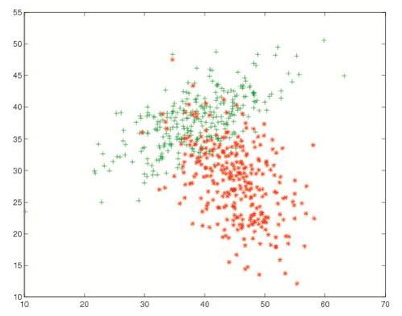
\includegraphics[width=0.45\textwidth]{pic/classification_plot.png}
%     %     \captionof{figure}{\scriptize [Sanja Fidler's Slides, University of Toronto, CSC411]}
%     % \end{center}
    
% \end{frame}
%%%%% 0.25 %%%%%%
% \begin{frame}{Probabilistic view in classification problem Cont.}
%     \begin{itemize}
%         \item Dataset visualization (x-axis denotes white blood count and y-axis represents plasma glucose value:
%     \end{itemize}
%     \begin{center}
%         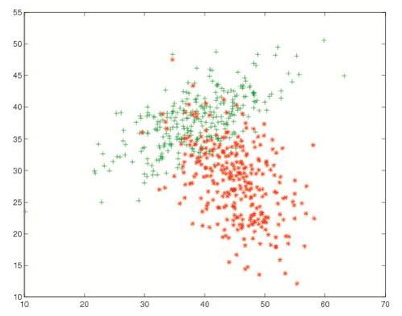
\includegraphics[width=0.45\textwidth]{pic/classification_plot.png}
%         \captionof{figure}{\footnotesize [Sanja Fidler's Slides, University of Toronto, CSC411]}
%     \end{center}
% \end{frame}

%%%%% 0.3 %%%%%
\begin{frame}{Probabilistic view in classification problem}
    \begin{itemize}
        \item In a classification problem:
            \begin{itemize}
                \item Each \textbf{feature} is a \textbf{random variable} (e.g. a person's height)
                \item The \textbf{class label} is also considered a \textbf{random variable} (e.g. a person could be overweight or not)
            \end{itemize}
        \item We observe the feature values for a random sample and intend to find its class label
            \begin{itemize}
                \item Evidence: Feature vector $x$
                \item Objective: Class label
            \end{itemize}
    \end{itemize}
\end{frame}
%%%%%0.5%%%%%%
\begin{frame}{Definitions}
    \begin{itemize}
        \item Posterior probability : The probability of a class label $C_k$ given a sample $x$
            \[
                P(C_k|x)
            \]
            
        \item Likelihood or class conditional probability : PDF of feature vector $x$ for samples of class $C_k$
            \[
                 P(x|C_k)
            \]
        
        \item Prior probability : Probability of the label be $C_k$ 
            \[
            P(C_k)
            \]
            
        \item $P(x)$: PDF of feature vector $x$ 
            \begin{itemize}
                \item From total probability theorem:   
                
                \[ P(x)=\sum_{k=1}^{K}P(x|C_k)P(C_k)
                \]
            \end{itemize}
        
    \end{itemize}
\end{frame}



%%% 1 %%%%
\subsection{Probabilistic classifiers}

\begin{frame}{Probabilistic classifiers}
    \begin{itemize}
        \item Probabilistic approaches can be divided in two main categories:
            \begin{itemize}
                \item Generative
                    \begin{itemize}
                        \item Estimate PDF $P(x, C_k)$ for each class $C_k$ and then use it to find $P(C_k|x)$. Alternatively estimate both PDF $P(x|C_k)$ and $P(C_k)$ to find $P(C_k|x)$.
                    \end{itemize}
                \item Discriminative
                    \begin{itemize}
                        \item Directly estimate $P(C_k|x)$ for class $C_k$
                    \end{itemize}
            \end{itemize}
    \end{itemize}
\end{frame}
%%%%%%%% 1.5 %%%%%%%%%%%%
\begin{frame}{Probabilistic classifiers (cont.)}
    \begin{itemize}
        \item Let's assume we have input data $x$ and want to classify the data into labels $y$.
        \item A generative model learns the \textbf{joint} probability distribution $P(x,y)$.
            
        \item A discriminative model learns the \textbf{conditional} probability distribution $P(y|x)$
           
    \end{itemize}
\end{frame}

%%%% 1.6 %%%%%%
\begin{frame}{Discriminative vs. Generative : example}
    \begin{itemize}
        \item Suppose we have the following dataset in form of $(x, y)$:
            \[
                (1,0), (1,0), (2,0), (2,1)
            \]
        \item $P(x,y)$ is :
            \[
            \begin{array}{c|cc}
                & y=0 & y=1 \\
                \hline
            x=1 & \frac{1}{2} & 0 \\
            x=2 & \frac{1}{4} & \frac{1}{4} \\
            \end{array}
            \]
        \item $P(y|x)$ is :
            \[
            \begin{array}{c|cc}
                & y=0 & y=1 \\
                \hline
            x=1 & 1 & 0 \\
            x=2 & \frac{1}{2} & \frac{1}{2} \\
            \end{array}
            \]
    \end{itemize}
\end{frame}

%%%%% 1.8 %%%%%

\begin{frame}{Discriminative vs. Generative : example (cont.)}
    \begin{itemize}
        \item The distribution $P(y|x)$ is the natural distribution for classifying a given sample $x$ into class $y$.
            \begin{itemize}
                \item This is why that algorithms which model this directly are called \textbf{discriminative} algorithms.
            \end{itemize}
        \item Generative algorithms model $P(x,y)$, which can be transformed into $P(y|x)$ by Bayes rule and then used for classification.
            \begin{itemize}
                \item However, the distribution $P(x,y)$ can also be used for other purposes.
                \item For example we can use $P(x,y)$ to \textbf{generate} likely $(x,y)$ pairs
            \end{itemize}
    \end{itemize}
\end{frame}

%%%% 2 %%%%%
\begin{frame}{Generative approach}
    \begin{enumerate}
        \item Inference
        \begin{itemize}
            \item Determine class conditional densities $P(x|C_k)$ and priors $P(C_k)$
            \item Use Bayes theorem to find $P(C_k|x)$
        \end{itemize}
        \item Decision
        \begin{itemize}
            \item Make optimal assignment for new input (after learning the model in the inference stage)
            \item if $P(C_i|x) > P(C_j|x) \forall j \neq i$, then decide $C_i$ .
        \end{itemize}
    \end{enumerate}
\end{frame}

%%%% 2.5 %%%%%
\begin{frame}{Generative approach (cont.)}

    \begin{itemize}
        \item Generative approach for a binary classification problem:
    \end{itemize}
    \begin{figure}[h]
      \centering
      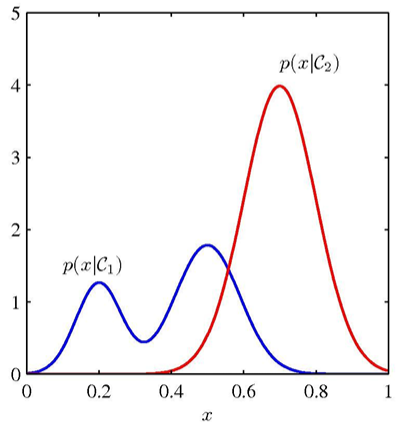
\includegraphics[width=0.4\textwidth]{pic/Generative.png}
    %   \caption*{\footnotesize [Bishop]}
      \end{figure}
    \vfill
    \begin{tikzpicture}[remember picture,overlay]
        \node[anchor=south west, xshift=0.1cm, yshift=0.22cm] at (current page.south west) {
            \scriptsize Figures adapted from Machine Learning and Pattern Recognition, Bishop
        };
    \end{tikzpicture}
\end{frame}
%%%% 3 %%%%
\begin{frame}{Discriminative approach}
    \begin{enumerate}
        \item Inference
        \begin{itemize}
            \item Determine the posterior class probabilities $P(C_k|x)$ directly.
        \end{itemize}
        \item Decision
        \begin{itemize}
            \item Make optimal assignment for new input (after learning the model in the inference stage)
            \item if $P(C_i|x) > P(C_j|x) \forall j \neq i$, then decide $C_i$ .
        \end{itemize}
    \end{enumerate}
\end{frame}
%%%% 3.5 %%%%%%
\begin{frame}{Discriminative approach (cont.)}
    \begin{itemize}
        \item Discriminative approach for a binary classification problem:
    \end{itemize}
    \begin{figure}[h]
      \centering
      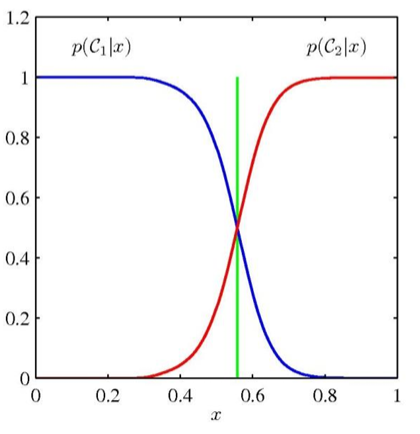
\includegraphics[width=0.4\textwidth]{pic/Disc.png}
    %   \caption*{\footnotesize [Bishop]}
      \end{figure}
    \vfill
    \begin{tikzpicture}[remember picture,overlay]
        \node[anchor=south west, xshift=0.1cm, yshift=0.22cm] at (current page.south west) {
            \scriptsize Figures adapted from Machine Learning and Pattern Recognition, Bishop
        };
    \end{tikzpicture}
\end{frame}
%%% 4 %%%%
    %% partition photos into 2 slides
% \begin{frame}{Discriminative vs. Generative approach}
%   \begin{figure}[h]
%   \centering
%   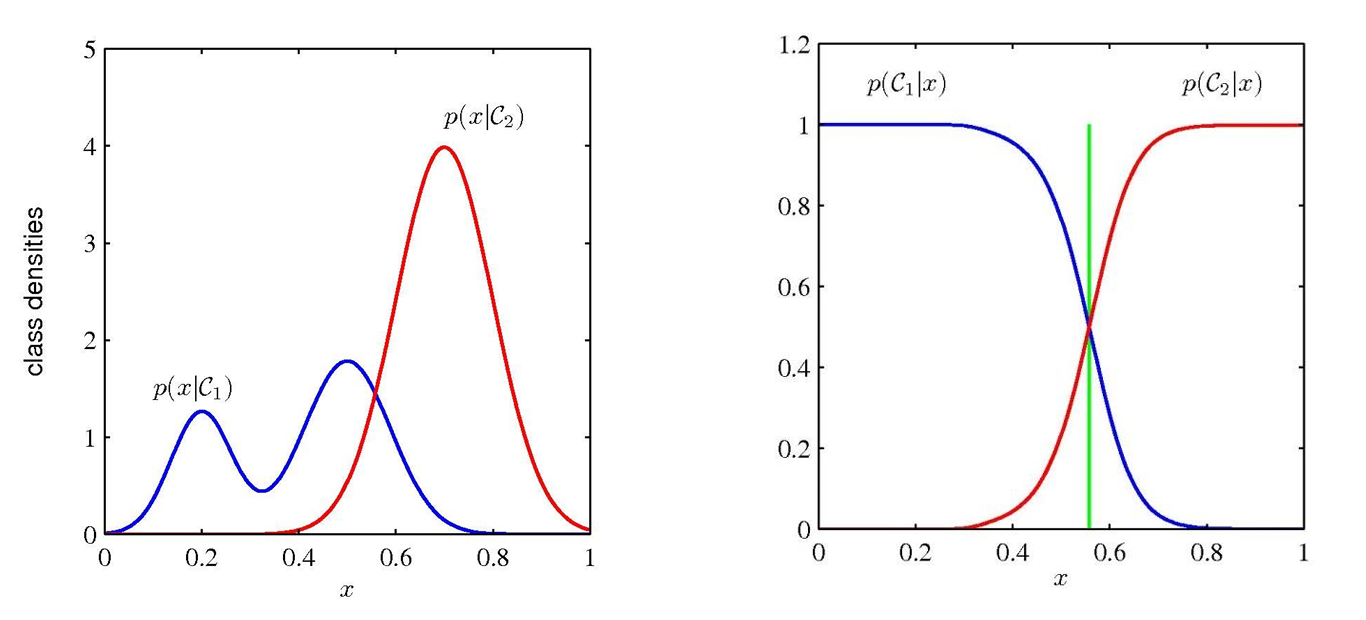
\includegraphics[width=\textwidth]{pic/GvD.png}
%   \caption*{[Bishop]}
%   % \label{fig:image}
% \end{figure}
% \end{frame}
\begin{frame}{Discriminative approach (cont.)}
    \begin{itemize}
        \item Logistic regression is a \textbf{discriminative} approach.
        \item We directly want to specify the class label with $\sigma (\mathbf{w}^T x)$
    \end{itemize}
\end{frame}

\section{References}

\begin{frame}{Contributions}
\begin{itemize}
\item \textbf{These slides are authored by:}
\begin{itemize}
    \setlength{\itemsep}{10pt} % Adjust the value to control the spacing
    \item \href{https://github.com/Danial-Gharib}{Danial Gharib}
\end{itemize}
\end{itemize}

\end{frame}

\begin{frame}[allowframebreaks]
    \bibliography{ref}
    \bibliographystyle{ieeetr}
    \nocite{*}
\end{frame}

\begin{frame}
    \begin{center}
        {\Huge Any Questions?}
    \end{center}
\end{frame}

\end{document}
